\documentclass{article}
\usepackage[T1]{fontenc}
\usepackage{lmodern}
\usepackage{graphicx}
\usepackage{amsmath,amssymb}
\usepackage[a4paper,margin=2cm]{geometry}
\usepackage[absolute,overlay]{textpos}
\setlength{\TPHorizModule}{1mm}
\setlength{\TPVertModule}{1mm}
\usepackage[indonesian]{babel}
\usepackage{hyperref}
\setlength{\emergencystretch}{2em}
% unit: Halaman 16

\begin{document}

% === Halaman 16 (llm) ===

\section*{Penggandaan Titik}

\vspace{181.17mm}

\begin{itemize}
    \item Penggandaan titik (\textit{point doubling}): menjumlahkan sebuah titik pada dirinya sendiri
    \vspace{10mm}
    \item Penggandaan titik membentuk tangen pada titik $P(x, y)$
    \item $P + P = 2P = R$
\end{itemize}

\vspace{5mm}
\textcolor{red}{Sumber gambar: Andreas Steffen, Elliptic Curve Cryptography}

% deskripsi: Grafik kurva eliptik yang mengilustrasikan operasi penggandaan titik (point doubling), menunjukkan garis tangen di titik P, titik potong R, dan refleksinya -R.
% bbox normalisasi: [0.4500, 0.2300, 0.8800, 0.8400]
\begin{textblock*}{90.30mm}(94.50mm,68.31mm)
\noindent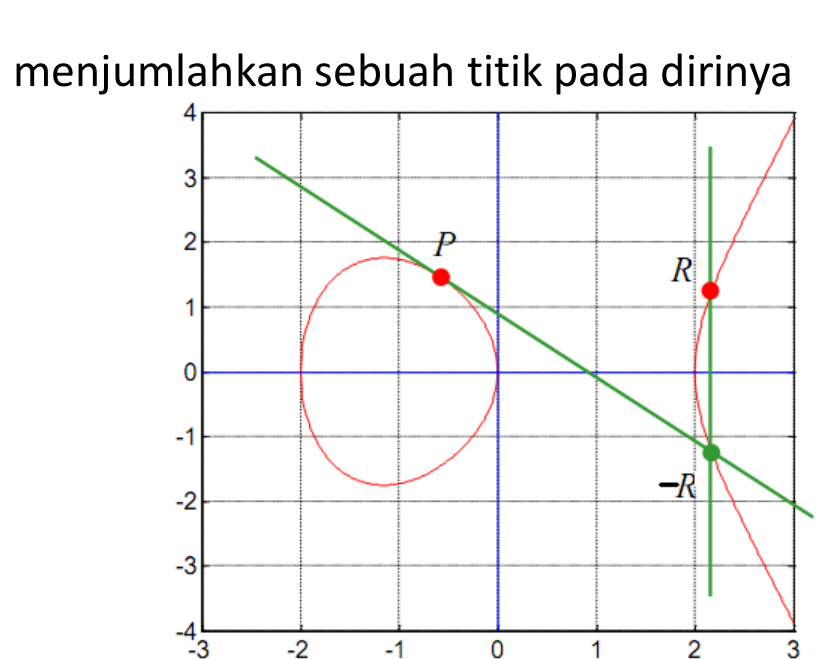
\includegraphics[width=90.30mm,height=181.17mm]{../../images/llm/page_016_img_01.png}%
\end{textblock*}

\end{document}
